
\begin{abstract}
    The computational sparsity of Mixture-of-Experts (MoE) models enables sub-linear growth in compute cost as
    model size increases, offering a scalable path to training massive neural networks.
    However, existing implementations suffer from \emph{low GPU utilization}, \emph{significant latency overhead},
    and a fundamental \emph{inability to leverage task locality},
    primarily due to CPU-managed scheduling, host-initiated communication, and frequent kernel launches.
    To overcome these limitations, we develop \sysname,
    a fully GPU-resident MoE operator that fuses expert computation and inter-GPU communication
    into a \emph{single persistent GPU kernel}.
    \sysname enables fine-grained pipelining of dispatch, compute, and combine phases,
    eliminating launch overheads and reducing idle gaps.
    Its device-initiated communication protocol introduces \emph{payload-efficient} data transfers,
    significantly shrinking buffer sizes in sparsely activated MoE layers.
    When evaluated on a single 8-H100 GPU node with MoE models having up to 128 experts and 16K token sequences,
    \sysname achieves up to \textbf{6}$\times$ lower latency, \textbf{5.7}$\times$ higher throughput,
    \textbf{4}$\times$ better overlap efficiency, and \textbf{9}$\times$ higher GPU utilization
    compared to state-of-the-art baselines—despite using FP32 while baselines use FP16.
    FlashDMoE demonstrates that principled GPU kernel-hardware co-design
    is key to unlocking the performance ceiling of large-scale distributed ML workloads.
\begin{figure}[!h]
    \centering
    \begin{subfigure}{0.4\textwidth}
        \centering
        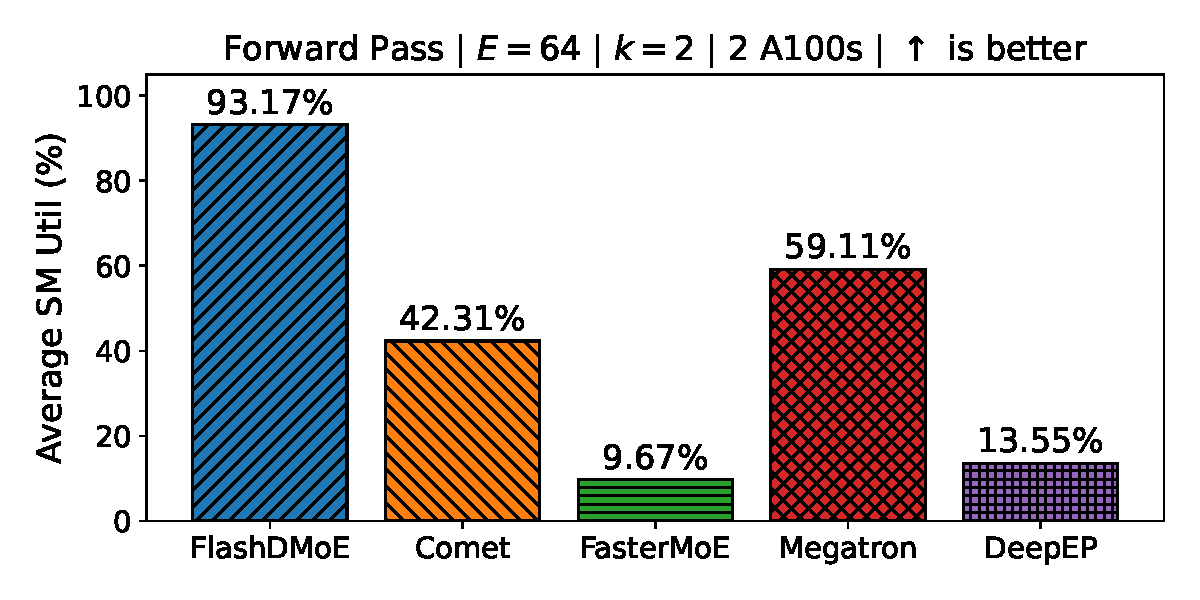
\includegraphics[width=\linewidth, keepaspectratio]{figures/sm_util}
        \caption{GPU SM Utilization}
        \label{sub:e}
    \end{subfigure}
    \begin{subfigure}{0.4\textwidth}
        \centering
        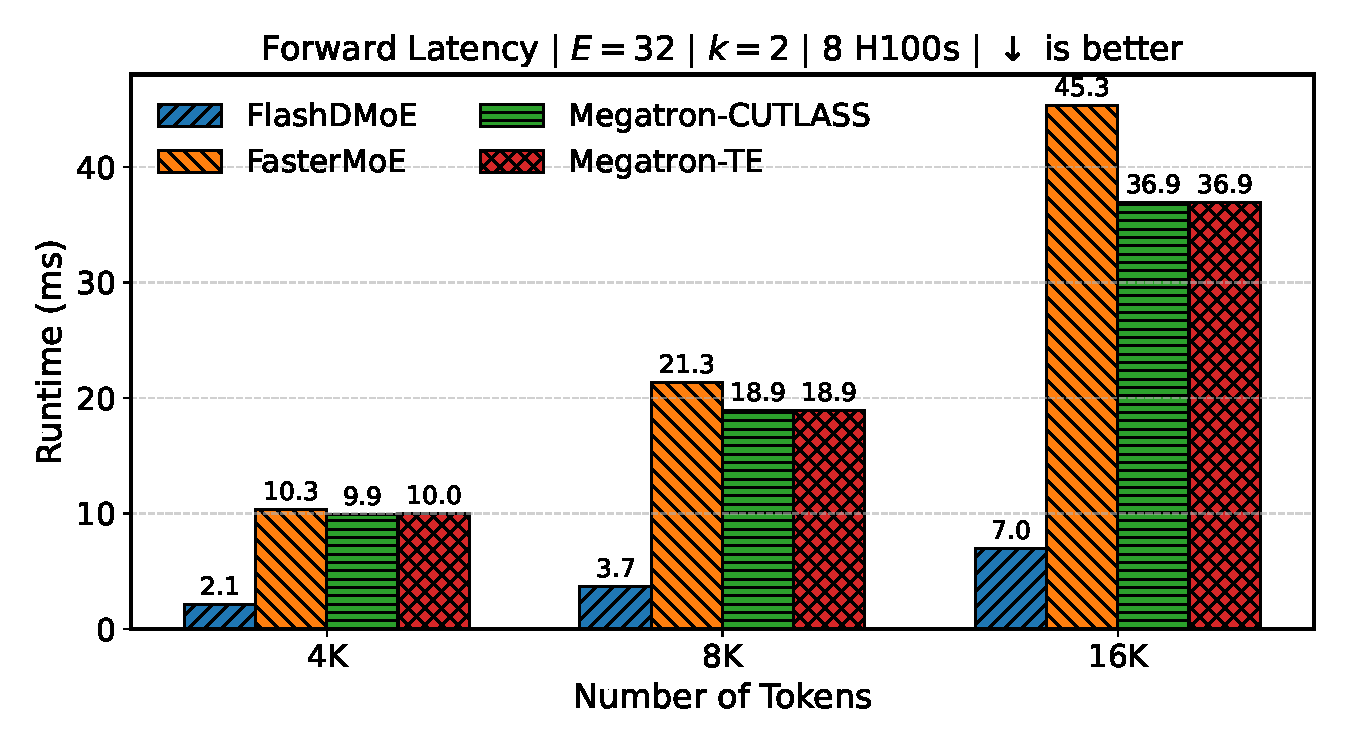
\includegraphics[width=\linewidth, keepaspectratio]{figures/scaling_tokens_8}
        \caption{Scaling Tokens}
        \label{sub:r}
    \end{subfigure}
    \begin{subfigure}{0.4\textwidth}
        \centering
        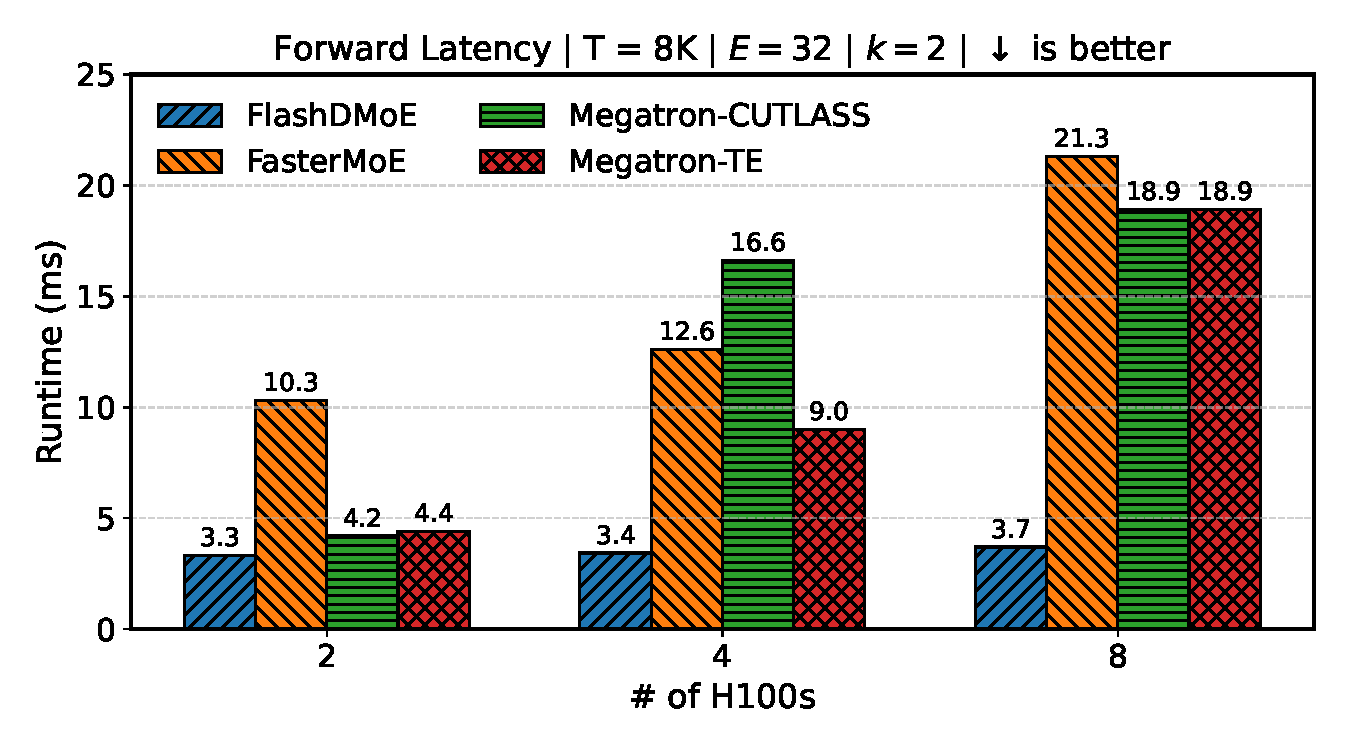
\includegraphics[width=\linewidth, keepaspectratio]{figures/scaling_gpus_8}
        \caption{Weak Scaling across GPUs}
        \label{sub:e1}
    \end{subfigure}
    \begin{subfigure}{0.4\textwidth}
        \centering
        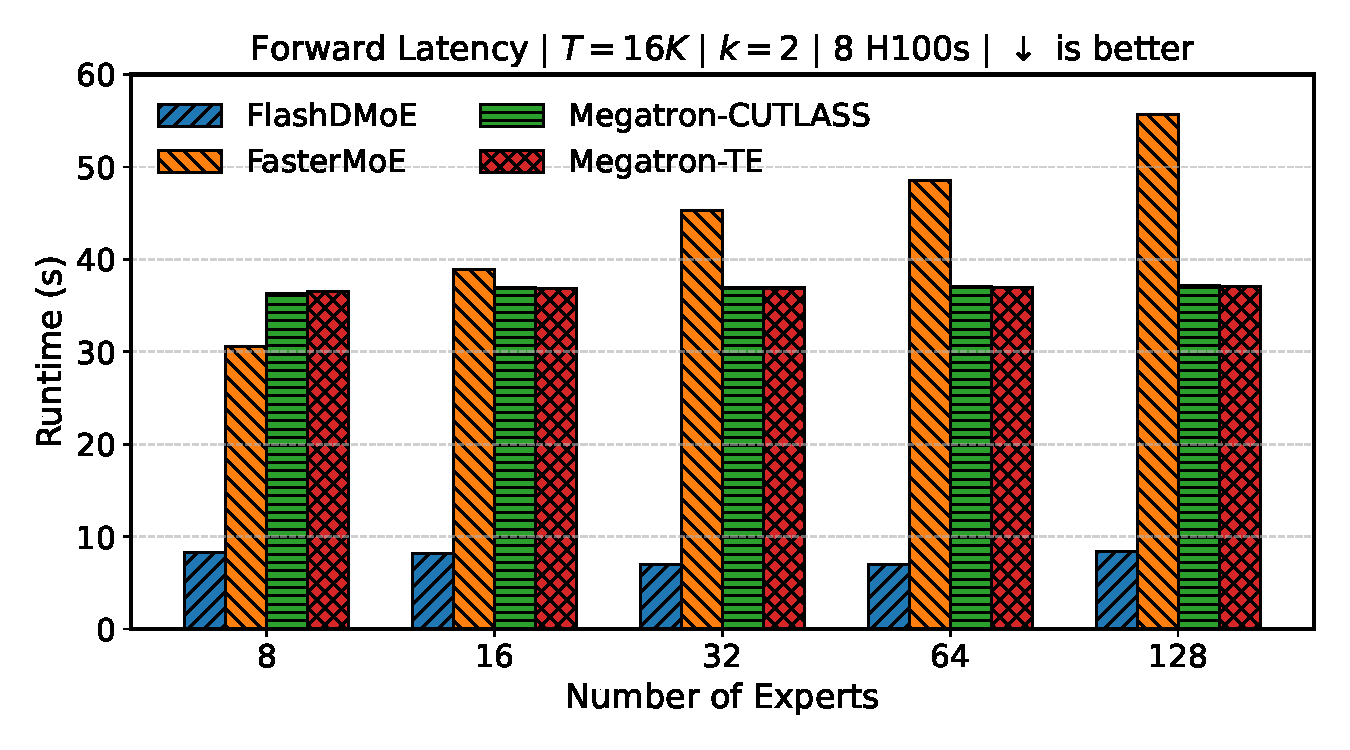
\includegraphics[width=\linewidth, keepaspectratio]{figures/scaling_experts_8}
        \caption{Across Experts}
        \label{sub:r2}
    \end{subfigure}
    \caption{\emph{FlashDMoE} performance.}
    \label{fig:str}
\end{figure}
\end{abstract}